\vspace{-.5cm}
\section{Tool Demonstration}
\label{sec:demo}
\vspace{-.3cm}
In this section, we discuss the main steps of the process that need to be
followed for synthesizing the EARS-CTRL specification into a controller and
validating if the controller behaves as expected.
\vspace{-.6cm}
\subsection{Building a Glossary}
\vspace{-.3cm}
The first step towards writing the controller specifications in natural
language using \textsf{EARS-CTRL} is to define a glossary of terms. 
As is depicted in figure~\ref{fig:glossary_def}, the user is provided with an
editor to define glossary terms for: \emph{A}) components that interface
with the controller; \emph{B}) sensors and actuators those components make
available to the controller; \emph{C}) invariant relations that should hold
between the sensor and actuator signals; and \emph{D}) for ease of writing,
aliases to formulas involving sensors or actuators.
\vspace{-.2cm}
\begin{figure*}[!h]
\centering
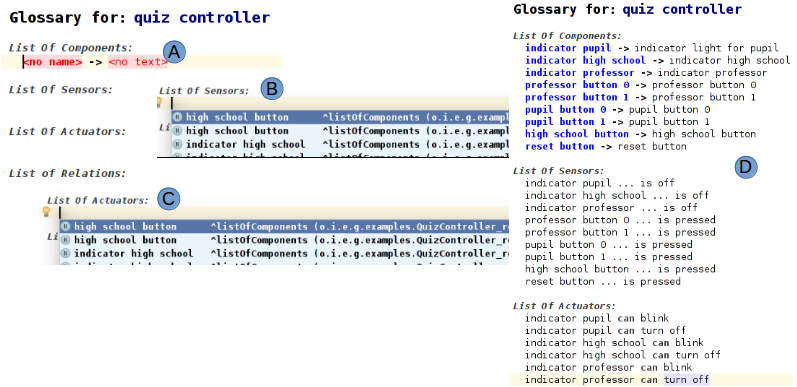
\includegraphics[width=1\textwidth]{./images/QC_Glossary_Def.png}
\caption{Step-by-step glossary building for a Quiz Controller: (\emph{A})
components definition, (\emph{B}) sensors definition, (\emph{C}) actuators
definition and (\emph{D}) completed QC glossary}
\label{fig:glossary_def}
\vspace{-.8cm}
\end{figure*}
\subsection{Building \textsf{EARS-CTRL} requirements for the Quiz Controller}
\vspace{-.2cm}
Figure~\ref{fig:EARS_req} provides the set of steps required to write a set of
EARS requirements. In the projectional editor the user presses the CTRL+Space
key combination to instantiate an EARS-based template that presents a number of
placeholders (\emph{Step A}). After obtaining
an instance of the EARS template, the user fills in the placeholders with
information coming from the glossary definitions (\emph{Step B}). \emph{Step C}
depicts the complete Quiz Controller specification.
\begin{figure*}[!h]
\centering
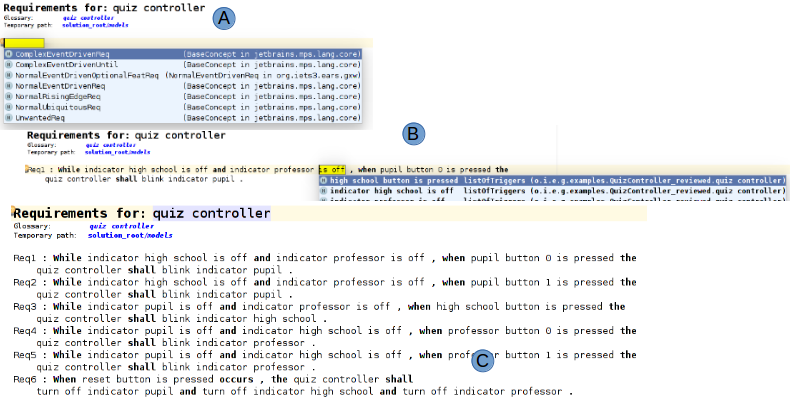
\includegraphics[width=1.2\textwidth]{./images/Req_Spec_Steps.png}
\caption{Step-by-step guidance for building controller requirements in
\textsf{EARS-CTRL}, (\emph{A}) empty instance of EARS template with placeholders, (\emph{B}) filling instance
of an EARS template with information and (\emph{C}) completed EARS Specification}
\label{fig:EARS_req}
%\vspace{-.8cm}
\end{figure*}
\vspace{-.2cm}
\subsection{Synthesizing \textsf{EARS-CTRL} requirements}
\label{SynthReq}
\vspace{-.3cm}
Once the requirements for controller are completely specified, the user can
attempt to synthesize the controller. For that the \emph{Transform} intention
can be used by using the \emph{Alt+Enter} keys on the root of the specification
(as shown in \emph{part A} of figure~\ref{fig:Spec_transform}). The generated
output after applying the intention is comprised of: \emph{B}) the 
\emph{Synchronized Data Flow} (SFD) diagram containing blocks connected by
wires; \emph{C}) pseudo code representing the behavior of each of the blocks
used by the synthesized controller; \emph{D}) a Simulink block
diagram; and \emph{E}) empty panel
for performing simulation and test cases generation.
%\vspace{-.7cm}
\begin{figure*}[!h]
\centering
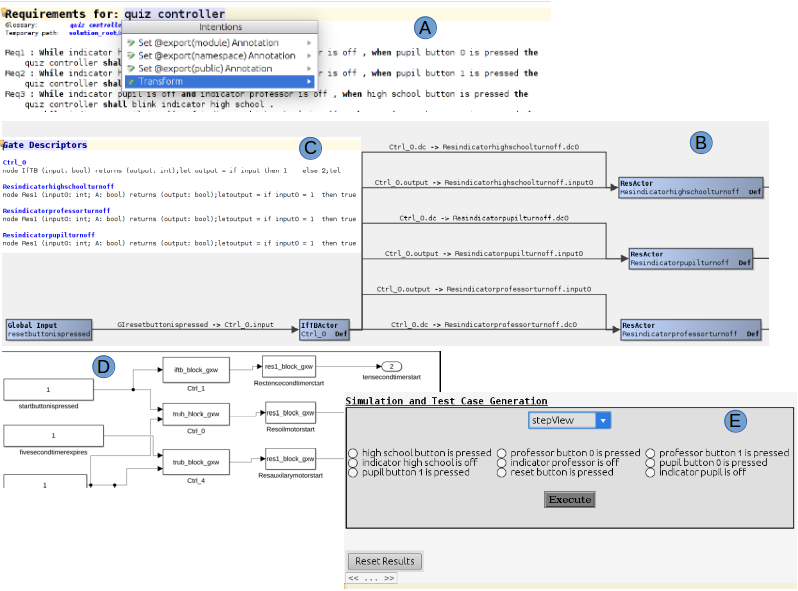
\includegraphics[width=1\textwidth]{./images/Transform.png}
\caption{Controller generation steps: (\emph{A}) applying intention \emph{Alt+Enter},
(\emph{B}) synchronized DFD of the controller (an excerpt), (\emph{C}) pseudo
code representing the behavior of the blocks (an excerpt), (\emph{D})
generated Simulink model (an excerpt) and (\emph{E})
generated empty panel for simulation}
\label{fig:Spec_transform}
\end{figure*}
%\vspace{-.5cm}
\subsection{Simulation and Test Cases for Validation of Controller
Behavior}
\vspace{-.2cm}
Validation of the generated controller can be performed using 1) simulation
and/or 2) test case generation.
\vspace{-.3cm}
\subsubsection{Simulation}
\vspace{-.2cm}
In order to perform simulation of the generated controller, the user is provided
with the \textsf{Simulation and Test Case Generation} panel in
\textsf{EARS-CTRL}. \textsf{Part A} in Figure~\ref{fig:PanelView} shows a
step-by-step view of the panel. For performing the step-by-step simulation, the
user performs the process that is as follows , 1) select the
\textsf{\emph{stepView}} from the drop down menu on the panel, 2) select (i.e.,
selection means putting value to 1) or deselect (i.e., deselect means putting input value to 0) the radio buttons to give the inputs for simulation and 3) press the execute button. The output is added to
the lower part of the  panel. 
\begin{figure*}[!h]
\centering
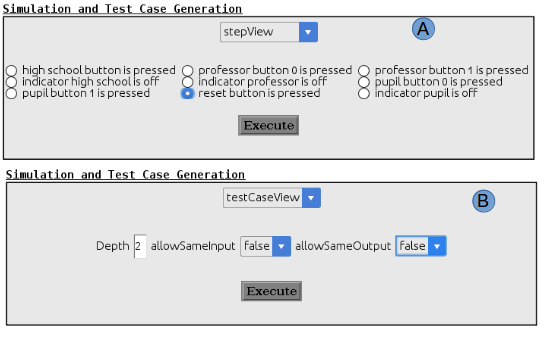
\includegraphics[width=.9\textwidth]{./images/Two_Views_Panel.png}
\caption{Simulation and test case generation panels, A) step-by-step simulation
view and B) test case generation view}
\label{fig:PanelView}
\vspace{-.4cm}
\end{figure*}
\vspace{-.4cm}
\subsubsection{Error Identification}
We selected the step-by-step view of the panel. We wanted to reset the
controller (execute the behavior of \emph{req6}in Figure~\ref{fig:QC_reqs}).
We executed req1 till req5 (steps not discussed in detail due to space limitation).
To simulate req6, we clicked the input
\textsf{\emph{reset Radio button is clicked}} on the panel (see \textsf{Part A}
in Figure~\ref{fig:PanelView}) and press the \emph{Execute} button. After
getting the result we expected all three outputs that are; 1) \emph{
indicator high school blink}, 2) \emph{indicator professor blink} and and 3)
\emph{indicator pupil blink in} to be set to the \emph{Off} state. But we
didn't get the expected behavior and the controller puts the indicator for the
pupil to the \emph{On} state as shown in Figure~\ref{fig:simError}. This
investigation led us to identify the error in \emph{req6} in
Figure~\ref{fig:QC_reqs}.
\begin{figure*}[!h]
\centering
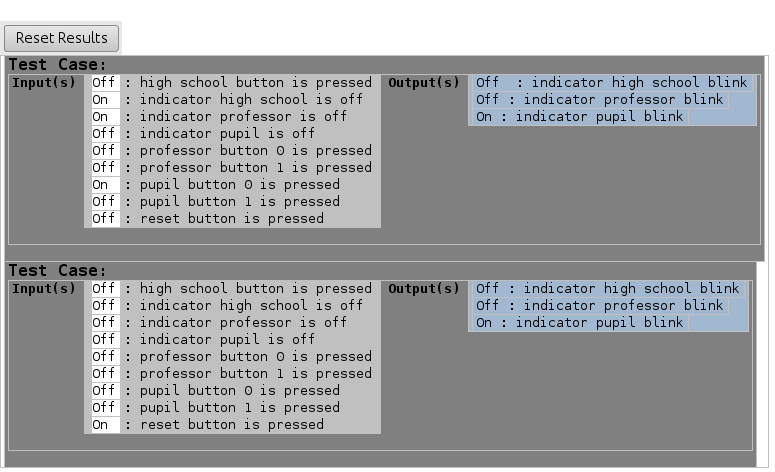
\includegraphics[width=.9\textwidth]{./images/Simulation_Error.png}
\caption{Error Identified during step-by-step simulation}
\label{fig:simError}
\vspace{-.6cm}
\end{figure*}
%\vspace{-.3cm}
\subsubsection{Automatic Test Cases Generation} 
\vspace{-.5cm}
\textsf{Part B} in Figure~\ref{fig:PanelView} shows a
test case generation view of the panel. For performing the test cases
generation, the user performs the process that is as follows, 1) select the
\textsf{\emph{testCaseView}} from the drop down menu on the panel, 2)
manually provides inputs for the simulation parameters (i.e., depth, allowSameInput and allowSameOutput) and 3) press the execute button. The output
is added to \textsf{Result checker} part of the panel.A \textsf{“Reset Results”} button enables the user to reset the controller to its initial state.
